\documentclass[a4paper,12pt]{amsart}

\usepackage{amsmath}
\usepackage{hyperref}
\usepackage{tikz}
\usepackage{tikz-3dplot}

\title{Introduction to vectors in three dimensions}

\begin{document}

\tdplotsetmaincoords{60}{120}

\maketitle
\tableofcontents

In this lesson we review the concepts of two-dimensional vectors covered in Unit 1 of Specialist Mathematics and extend to three dimensions.

\section{Definitions and notation}

\subsection{Vectors as directed line segments}

A \textbf{vector} is a quantity with both magnitude \emph{and} direction. Vectors can be represented in two or three dimensions as arrows oriented in the vector's direction whose length is the magnitude. An example in two and three dimensions is pictured below.

\[ 
    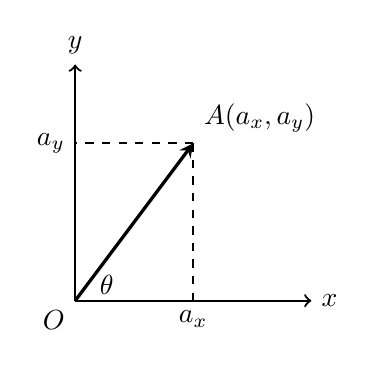
\begin{tikzpicture}[axis/.style={->,thick},
        vector/.style={-stealth,very thick},
        vector guide/.style={dashed,thick}]]
    \draw[axis] (0,0) -- (0,3) node[anchor=south] {$y$};
    \draw[axis] (0,0) node[anchor=north east] {$O$} -- (3,0) node[anchor=west] {$x$};
    \draw[vector] (0,0) -- (1.5,2) node[anchor=south west] {$A(a_x, a_y)$};
    \draw[vector guide] (1.5,2) -- (1.5,0) node[anchor=north] {$a_x$};
    \draw[vector guide] (1.5,2) -- (0,2) node[anchor=east] {$a_y$};
    \node at (0.4,0.2) {$\theta$};
    \end{tikzpicture} \qquad
    \begin{tikzpicture}[tdplot_main_coords,
        axis/.style={->,thick},
        vector/.style={-stealth,very thick},
        vector guide/.style={dashed,thick}]
    
        \coordinate (O) at (0,0,0);
        \tdplotsetcoord{P}{3}{55}{60};
    
        \draw[axis] (O) -- (3,0,0) node[anchor=north east] {$x$};
        \draw[axis] (O) -- (0,3,0) node[anchor=north west] {$y$};
        \draw[axis] (O) -- (0,0,3) node[anchor=south] {$z$};
        \draw[vector] (O) -- (P) node[anchor=south west] {$A(a_x, a_y, a_z)$};
        \draw[vector guide] (O) -- (Pxy);
        \draw[vector guide] (P) -- (Pxy);
        \draw[vector guide] (Px) node[above left] {$a_x$} -- (Pxy) -- (Py) node[above right] {$a_y$};
        \draw[vector guide] (P) -- (Pz) node[left] {$a_z$};
    \end{tikzpicture}
\]

\subsection{Naming vectors}

A vector whose tail is at the point $A$ and whose head is at the point $B$ is denoted by $\vec{AB}$. Vectors are also often denoted by a single bold lowercase letter. It is also common to use bold text with a lower case letter to denote a vector. For example, we may write $\mathbf{v} = \vec{AB}$. When handwriting, it can be challenging to distinguish bold text from normal, so it is common to write a tilde under the lowercase letter, like $\underset{\sim}{v}$. The images above show the vector $\vec{OA}$ which joins the origin, $O$, to a point $A$. For vectors whose tail is at the origin, we will often use the lower case letter corresponding to the head of the vector, like $\mathbf{a} = \vec{OA}$.

\subsection{Equality of vectors}

Two vectors are \textbf{equal} if they have the same magnitude \emph{and} direction, regardless of where they sit in space.  For example, in the image below all the vectors have the same magnitude. $\vec{AB}$ and $\vec{CD}$ are equal, but $\vec{EF}$ is different, since it points in a different direction.

\[
    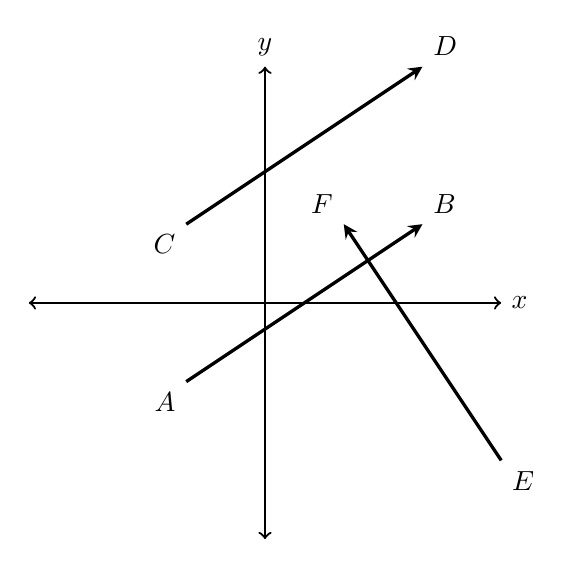
\begin{tikzpicture}[axis/.style={<->,thick},
        vector/.style={-stealth,very thick},
        vector guide/.style={dashed,thick}]]
    
        \draw[axis] (-3,0) -- (3,0) node[anchor=west] {$x$};
        \draw[axis] (0,-3) -- (0,3) node[anchor=south] {$y$};
    
        \coordinate (A) at (-1,-1);
        \coordinate (B) at (2,1);
        \coordinate (C) at (-1,1);
        \coordinate (D) at (2,3);
        \coordinate (E) at (3,-2);
        \coordinate (F) at (1,1);
        \draw[vector] (A) node[anchor=north east] {$A$} -- (B) node[anchor=south west] {$B$};
        \draw[vector] (C) node[anchor=north east] {$C$} -- (D) node[anchor=south west] {$D$};
        \draw[vector] (E) node[anchor=north west] {$E$} -- (F) node[anchor=south east] {$F$};
    \end{tikzpicture}
\]

\subsection{Column vectors}

We can write the vector $\vec{AB}$ in the diagram as a $2\times1$ matrix, or \textbf{column vector} $\begin{pmatrix} 4 \\ 3 \end{pmatrix}$.

\[
    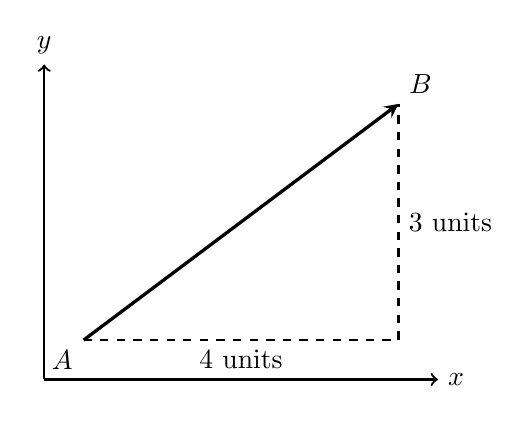
\begin{tikzpicture}[axis/.style={->,thick},
        vector/.style={-stealth,very thick},
        vector guide/.style={dashed,thick}]]
    
        \draw[axis] (0,0) -- (0,4) node[anchor=south] {$y$};
        \draw[axis] (0,0) -- (5,0) node[anchor=west] {$x$};
    
        \coordinate (A) at (0.5,0.5);
        \coordinate (B) at (4.5,3.5);
        \coordinate (C) at (4.5,0.5);
        \draw[vector] (A) node[anchor=north east] {$A$} -- (B) node[anchor=south west] {$B$};
        \draw[vector guide] (A) -- (C) node[midway, below] {4 units} -- (B) node[midway, right] {3 units};
    \end{tikzpicture}
\]

More generally, the column vector $\begin{pmatrix} x \\ y \end{pmatrix}$ represents a directed line segment which goes horizontally by $|x|$ units and vertically by $|y|$ units. The orientation of the vector is given by the sign of the component. Positive relates to right and up, and negative to left and down. In three dimensions we simply add a third component for the $z$ direction: $\begin{pmatrix} x \\ y \\ z \end{pmatrix}$.

\subsection{Magnitude}

The \textbf{magnitude}, $\left| \vec{AB} \right|$ of the vector $\vec{AB}$ in the diagram above is represented by the length of the arrow. It can therefore be calculated by Pythagoras' theorem

\[ \left| \vec{AB} \right| = \sqrt{4^2 + 3^2} = 5. \]

For two dimensions in general, a vector $\textbf{v} = \begin{pmatrix} x \\ y \end{pmatrix}$ is given by

\[ \left| \mathbf{v} \right| = \sqrt{x^2 + y^2}. \]

For three dimensions, it is just the three dimensional analogue of Pythagoras' theorem:
\[ \mathbf{v} = \begin{pmatrix} x \\ y \\ z \end{pmatrix} \implies \left| \mathbf{v} \right| = \sqrt{x^2 + y^2 + z^2}. \]

\end{document}